\documentclass{standalone}
\usepackage{pgfplots}
\usetikzlibrary{decorations.pathmorphing,patterns}
\begin{document}
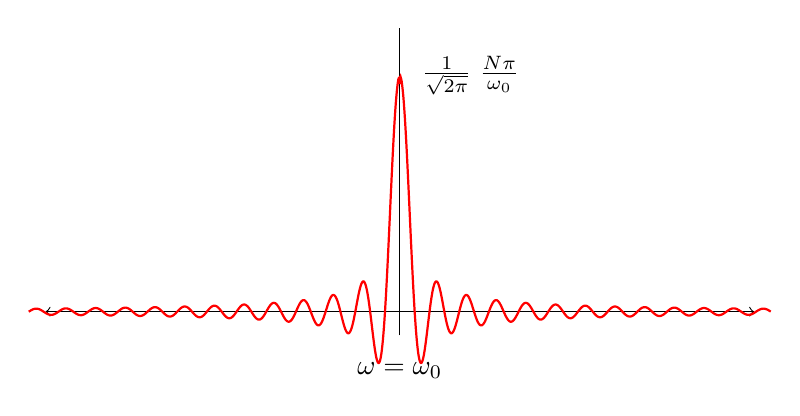
\begin{tikzpicture}[scale=3]
 	\draw[<->] (-1.5,0) -- (1.5,0);
  	\draw (0,-0.1)--(0,1.2);
    %\draw[very thin,color=gray] (-0.1,-1.1) grid (3.9,3.9);
	%\draw[color=blue]   plot (\x,{sin(\x r)}) ; 
	%\draw[domain=-20:20,samples=200,blue] plot(\x,{sqrt{2/pi}* (sin \x}* pi);
	\draw[red, thick] plot[domain = -pi/2:+pi/2, samples = 2000] (\x,{0.02*sin(50*(\x) r)/(\x))});	
	\draw (0,-0.25) node {$\omega = \omega_{0}$};
	\draw (0.3,1) node {$ \frac{1}{\sqrt{2 \pi}} \; \frac{N \pi}{\omega_{0}}$};
\end{tikzpicture}
\end{document}